\subsection{ET Proxy}
\begin{itemize}
	\item Proxy de Entrada (squid): O proxy de entrada tem a função de autenticar utilizadores, gerir os acessos e encaminhar os pedidos para o sistema de filtragem de conteúdos ou então para o proxy de saída.
	\item Filtro de Conteúdos (dansguardian): O filtro de conteúdos tem a funcção de verificar se os conteúdos pedidos pelo utilizador respeitam as normas definidas ou não.
	\item Proxy de Saída (squidsaida): O proxy de saída tem a função apenas de guardar uma \emph{cache}, ou seja, armazenar páginas ou partes das mesmas para acelerar a visualização aos utilizadores.
\end{itemize}

A configuração do proxy está acessível através da interface Web de gestão.
Este acesso permite modificar as regras de proxy e configurar aspectos de rede relativos ao servidor.

Todas as configurações do Proxy podem ser encontradas em \emph{/etc/squid} e \emph{/etc/dansguardian} e futuras referências a ficheiros de configuração vão partir deste pressuposto.

De modo a implementar as políticas definidas na definição de requisitos foi criado um sistema com o seguinte esquema:

\begin{figure}[H]
        \begin{center}
                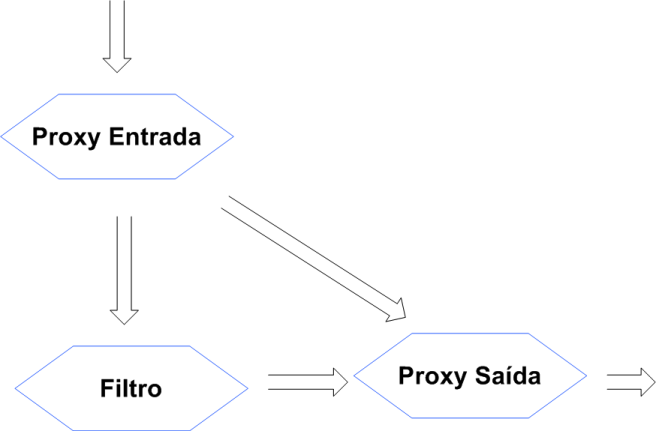
\includegraphics[width=11cm]{include/img/squid+dansguardian+squidsaida}
        \end{center}
        \caption{Diagrama Proxy}
        \label{fig:proxy}
\end{figure}

O funcionamento global da solução é o seguinte: quando um utilizador faz um pedido ao proxy é validada a sua autenticação e seguindo as regras definidas vai encaminhar o pedido ou para a filtragem ou para o proxy de saída.
No caso de ser encaminhado para a filtragem o conteúdo é filtrado de acordo com as regras definidas no programa.
Os pedidos são sempre feitos para a servidor destino utilizando o proxy de saída.
Deste modo faz-se a cache de conteúdo.

Uma vez que a filtragem necessita que o conteúdo esteja todo acessível leva a que o \emph{browser} tenha um aumento no tempo de resposta inicial mas que posteriormente se tornará mais rápido à medida que o proxy de saída vai armazenando informação.

% falta fazer o reset
%\renewcommand{\subsection}{\subsubsection}
\makeservice{squid}

\makeservice{dansguardian}
